\documentclass[11pt,a4paper]{article}
\usepackage[margin=1.7cm]{geometry}
\usepackage{fontspec,xeCJK}
\setmainfont{TeX Gyre Heros}
\setCJKmainfont{Noto Sans CJK SC}
\usepackage{graphicx,xcolor,tabularx,booktabs,enumitem}
\definecolor{Blue}{HTML}{153E63}
\definecolor{Gray}{HTML}{4B5966}
\definecolor{Pale}{HTML}{EDF4F7}
\usepackage[most]{tcolorbox}
\pagestyle{empty}
\setlength{\parindent}{0pt}
\setlength{\parskip}{5pt}
\begin{document}
{\small\color{Gray}《智慧水利平台架构与开发》\hfill 导学图 · 01}
\par\vspace{5pt}
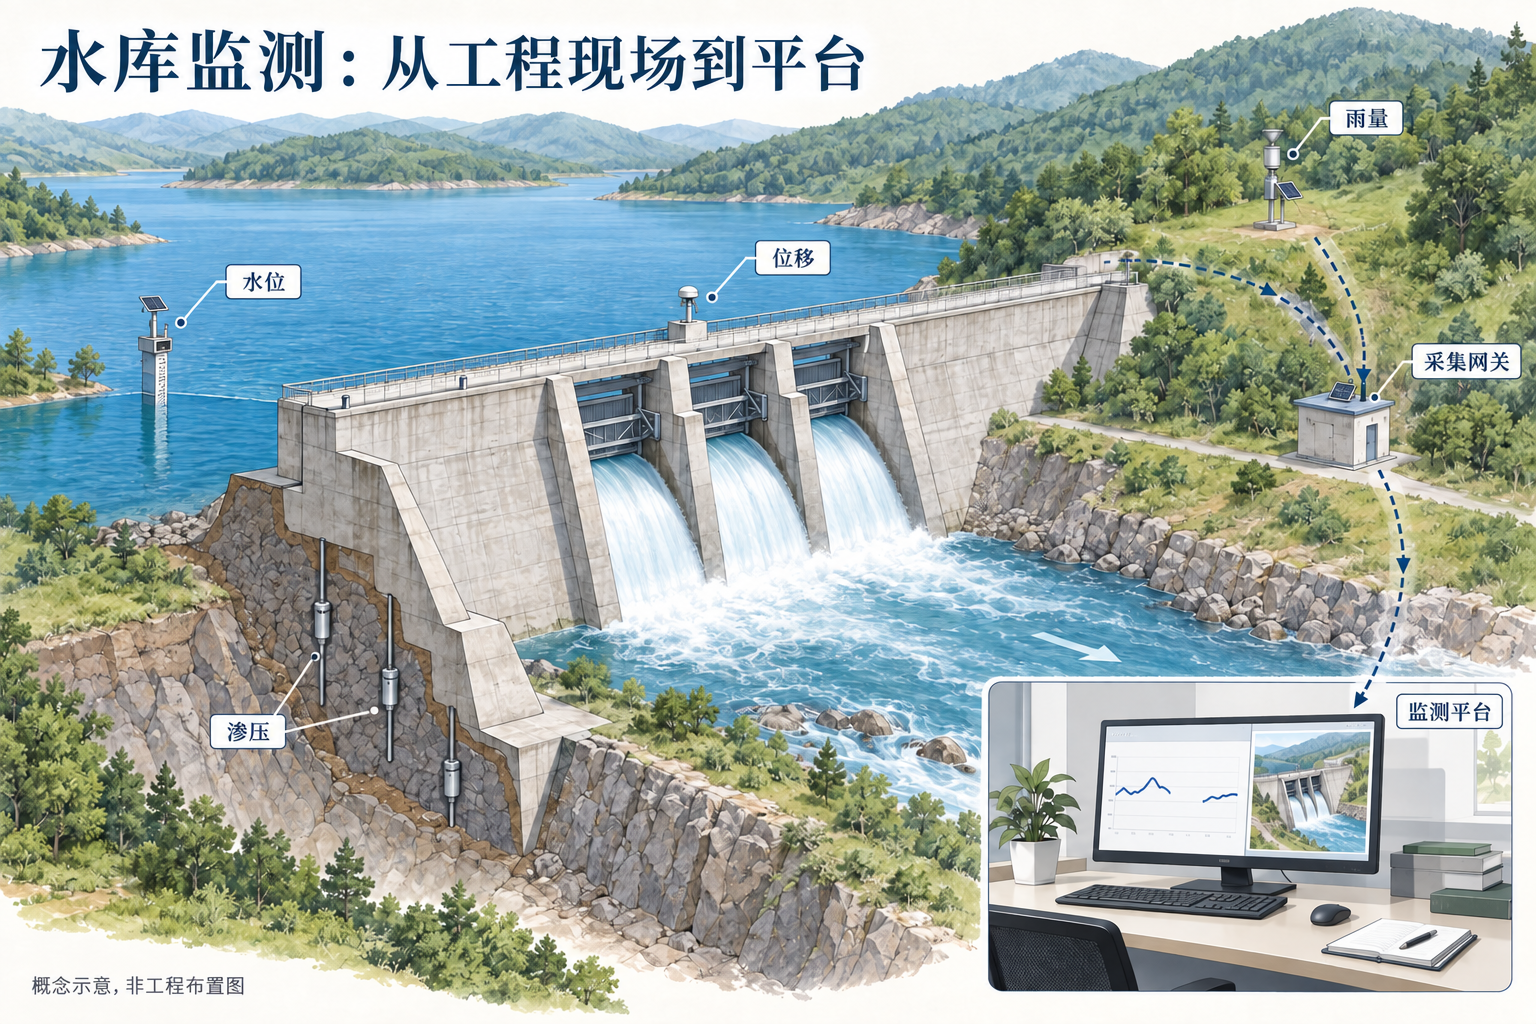
\includegraphics[width=\linewidth]{reservoir-monitoring-overview.png}
\par\vspace{8pt}
{\Large\bfseries\color{Blue}沿一条观测记录读图}
\par\vspace{5pt}
\renewcommand{\arraystretch}{1.35}
\begin{tabularx}{\linewidth}{@{}p{1.25cm}X p{2.3cm}@{}}
\toprule
环节 & 观察与解释 & 对应内容\\
\midrule
现场 & 找到水位、雨量、位移与渗压测点，说明各自观察的工程现象。图中仅示代表性位置。 & 第1、8章\\
传递 & 沿蓝色虚线找到网关与平台。观测记录需携带对象标识、时间、数值、单位与质量码。 & 第4、5章\\
展示 & 将测点绑定到三维对象，点击对象查询对应记录；图表与模型应使用同一对象标识。 & 第6、7章\\
处置 & 可用观测经规则判定形成预警；值班员确认并发起工单，高风险处置须由审批人批准。 & 第8章\\
\bottomrule
\end{tabularx}
\vspace{9pt}
\begin{tcolorbox}[colback=Pale,colframe=Pale,boxrule=0pt,arc=2pt,left=10pt,right=10pt,top=7pt,bottom=7pt]
{\bfseries\color{Blue}故障观察：曲线为什么断开？}\par
网关中断期间，平台收不到新观测。补齐时间格网并保留空值后，曲线在缺测位置断开。删掉空值再连线，会使读者误以为这段时间仍有连续观测。\par
{\bfseries 可观察结果：}曲线出现空缺，详情可查最后一次有效时间与缺测原因。\par
{\bfseries 自测：}曲线缺测能否判为“无预警”？\par
{\bfseries 答案要点：}不能。证据不足时显示“未评估”，同时保留历史结果的时间与有效期，核查链路状态。
\end{tcolorbox}
\vfill
{\footnotesize\color{Gray}读图提示：水流箭头与数据虚线含义不同。案例工程参数与监测数量以8.1节为准；本页为概念学习素材。}
\end{document}
